To evaluate the efficacy of each approach, a number of experiments are carried out. These experiments take the form of training the agent networks on a particular map, and testing the model every so often by measuring the win rate against the opponent. We hope to see a large maximum win rate, but also it is also beneficial to reach this maximum win rate faster. 

The particular maps contain a set of units for either team, with one team composed of the agents, and the other controlled by the built-in AI on ``very hard'' difficulty (which is the hardest built-in non-cheating AI difficulty).

The specific maps we will use in experiments are shown in the table below.

\vspace{3mm}
\begin{tabular}{ |p{2.5cm}||p{6.6cm}|  }
 \hline
 Map Name& Description\\
 \hline
 3m   & 3 marines on either team\\
 \hline
 2s3z   & 2 Stalkers and 3 Zealots on either team\\
 \hline
\end{tabular}

\subsection{Baseline Experiments}

The first set of experiments will be used to evaluate the performance of each candidate agent network architecture on different Starcraft II maps, namely 3m and 2s3z. This will give a baseline of performance on a simple map between for each candidate architecture. Each agent network is trained until it converges, with a test performed every 20,000 time steps to evaluate performance at that time. Each agent is trained a total of 5 times to allow for reproducible results and an evaluation of both the mean and variance of the test win rate will be made. Both the QMIX and VDN mixing networks will be used to allow us to compare the agent networks' performance using each mixing network.

In each experiment, the observation (and action) grid size) will be set to the maximum size that memory restraints allow (~6Gb, which allows two experiments per GPU). This is to evaluate the best possible performance of each agent under reasonable memory restrictions. In the 3m map, this grid size is $24 \times 24$.


\subsubsection{Baseline Experiments on 3m}

Firstly we shall evaluate the agents in the 3m map (3 marines on either team) using the VDN mixing network. We can see the performance of each agent network compared to the standard rnn agent network in figures \ref{fig:all_agents_3m_vdn_a} and \ref{fig:all_agents_3m_vdn_b}. In each of the graphs in this section, we shall only include a small number of agent networks architectures (to ensure each graph is clear), and we will always include the standard rnn to allow for comparison. In figure \ref{fig:all_agents_3m_vdn_a}, we can see that both conv\_input\_flat and rnn\_input learn at a similar rate to the standard rnn agent network, reaching a similar maximum test win rate of 95+\%. However, in figure \ref{fig:all_agents_3m_vdn_b}, it is clear that both the conv\_input\_grid and conv architectures learn at a quicker rate than the standard rnn agent network, increasing to around an 80\% test win rate after just 750,000 time steps, whereas the standard rnn agent network reaches just 60\% in this time. All agent networks do, however, converge at around a 90\% test win rate at 1,250,000 time steps, before converging to the same maximum test win rate of 95+\%.

The same experiment is run using the QMIX network, as shown in figures \ref{fig:all_agents_3m_qmix_a} and \ref{fig:all_agents_3m_qmix_b}. Again, all agents perform well, each reaching at least 40\% test win rate after just 100,000 time steps. Furthermore, each agent reaches 95+\% win rate by around 1,250,000 time steps. The conv\_input\_flat architecture both perform similar to the standard rnn architecture, but both the conv and conv\_input\_grid architectures can be seen to converge slightly earlier, at just 1,000,000 time steps, when compared to the standard rnn architecture.

\begin{figure}[!tbp]
  \centering
  \subfloat[Test win rate of conv\_input\_flat, rnn\_input and rnn architectures.]{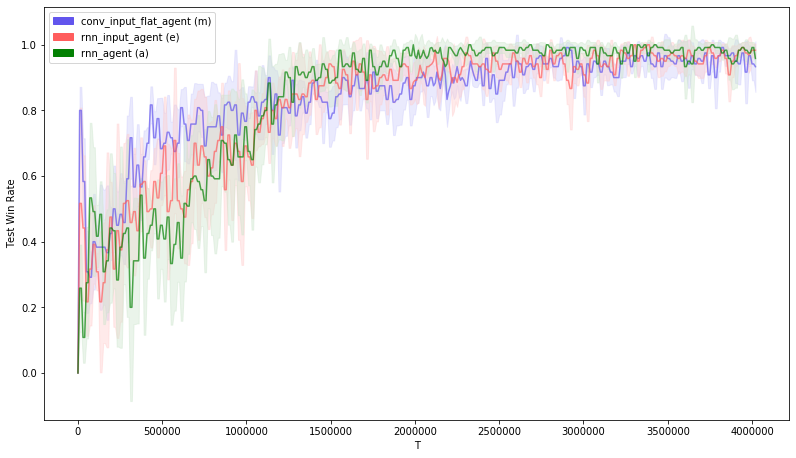
\includegraphics[width=0.45\textwidth]{images/graphs/allagents/3m_vdn_1.png}\label{fig:all_agents_3m_vdn_a}}
  \hfill
  \subfloat[Test win rate of conv\_input\_grid, conv and rnn architectures.]{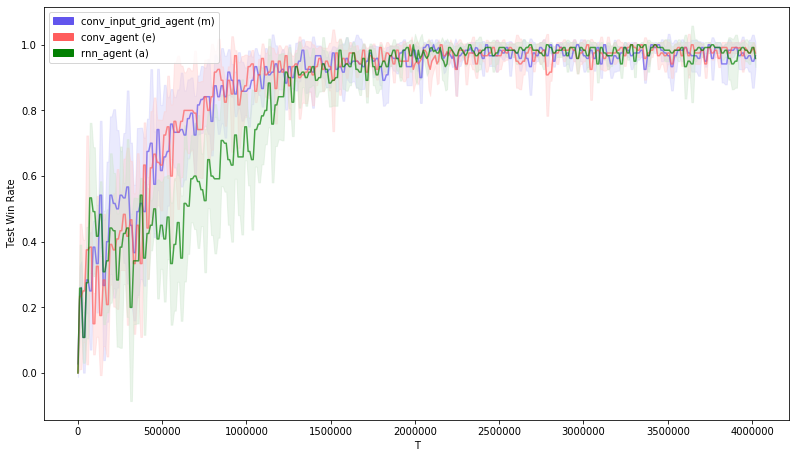
\includegraphics[width=0.45\textwidth]{images/graphs/allagents/3m_vdn_2.png}\label{fig:all_agents_3m_vdn_b}}
  \caption{Test win rate of each candidate network architecture on the 3m map with the VDN mixing network.}
\end{figure}

\begin{figure}[!tbp]
  \centering
  \subfloat[Test win rate of conv\_input\_flat, rnn\_input and rnn architectures.]{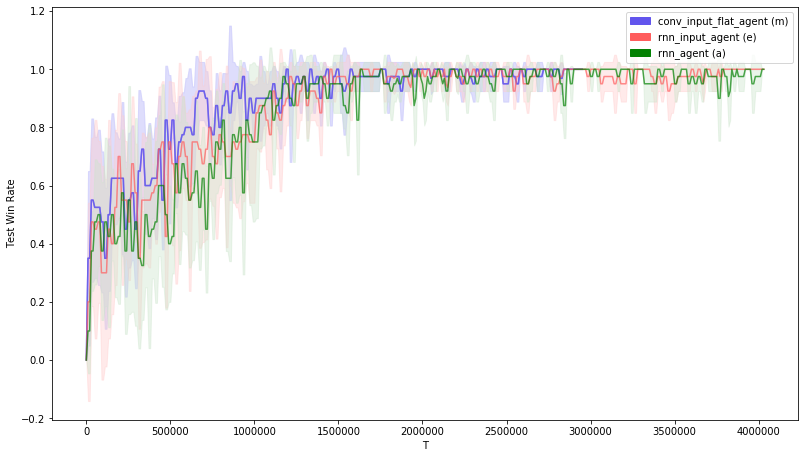
\includegraphics[width=0.45\textwidth]{images/graphs/allagents/3m_qmix_1.png}\label{fig:all_agents_3m_qmix_a}}
  \hfill
  \subfloat[Test win rate of conv\_input\_grid, conv and rnn architectures.]{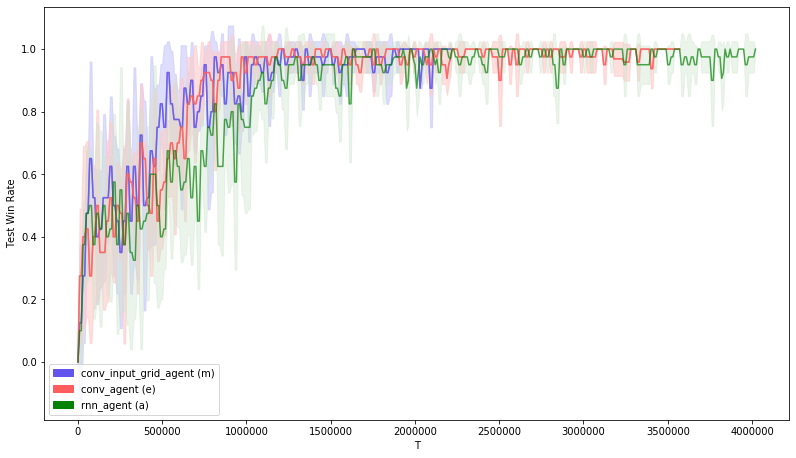
\includegraphics[width=0.45\textwidth]{images/graphs/allagents/3m_qmix_2.png}\label{fig:all_agents_3m_qmix_b}}
  \caption{Test win rate of each candidate network architecture on the 3m map with the QMIX mixing network.}
\end{figure}

\subsubsection{Baseline Experiments on 2s3z}
Next, we run the same set of  experiments on the 2s3z map (2 Stalkers and 3 Zealots on either team) on both the VDN and QMIX mixing networks. Clearly, the QMIX mixing network appears to be superior to VDN in the 2s3z environment. This is shown by a larger maximum win rate for all agent architectures (each agent's maximum win rate is at least 10-20\% greater with QMIX compared to VDN), and each agent converges far more quickly.

The conv\_input\_grid architecture did best overall (using both the VDN and QMIX mixing network). The architecture exhibited a very high initial rate of learning (especially in the QMIX network), before converging at over 90\% test win rate in both VDN and QMIX. This architecture was consistently better than the standard rnn architecture.

The conv architecture also performed fairly well, paritcularly in the QMIX network. It had very similar performance to the standard rnn architecture in QMIX, but had a slower rate of learning (and reached a slightly lower maximum win rate) in the VDN network.

Both the conv\_input\_flat and rnn\_input\_flat performed poorly on this map, consistently having a lower test win rate at each timestep when compared to the standard rnn architecture. In the VDN network, after 10 million timesteps the architectures had not yet converged. The experiment was stopped at this point as this training time is unreasonable. In the QMIX network, both reached a final test win rate of just over 80\%, which is poor considering the time spent training.

\begin{figure}[!tbp]
  \centering
  \subfloat[Test win rate of conv\_input\_flat, rnn\_input and rnn architectures.]{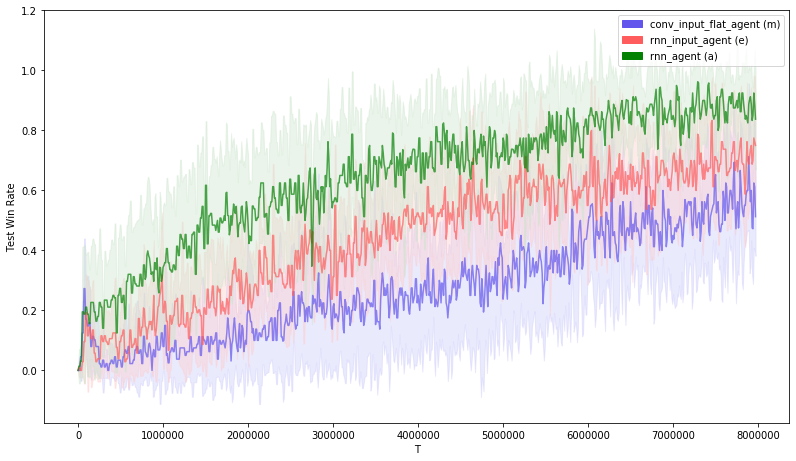
\includegraphics[width=0.45\textwidth]{images/graphs/allagents/2s3z_vdn_1.png}\label{fig:all_agents_2s3z_vdn_a}}
  \hfill
  \subfloat[Test win rate of conv\_input\_grid, conv and rnn architectures.]{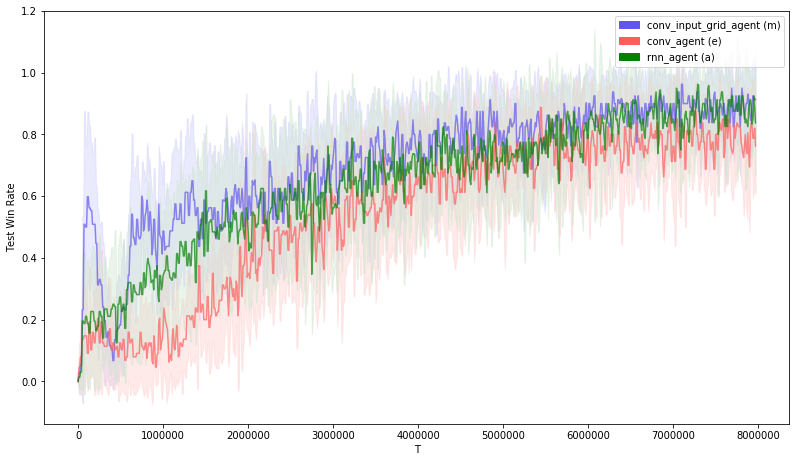
\includegraphics[width=0.45\textwidth]{images/graphs/allagents/2s3z_vdn_2.png}\label{fig:all_agents_2s3z_vdn_b}}
  \caption{Test win rate of each candidate network architecture on the 2s3z map with the VDN mixing network.}
\end{figure}

\begin{figure}[!tbp]
  \centering
  \subfloat[Test win rate of conv\_input\_flat, rnn\_input and rnn architectures.]{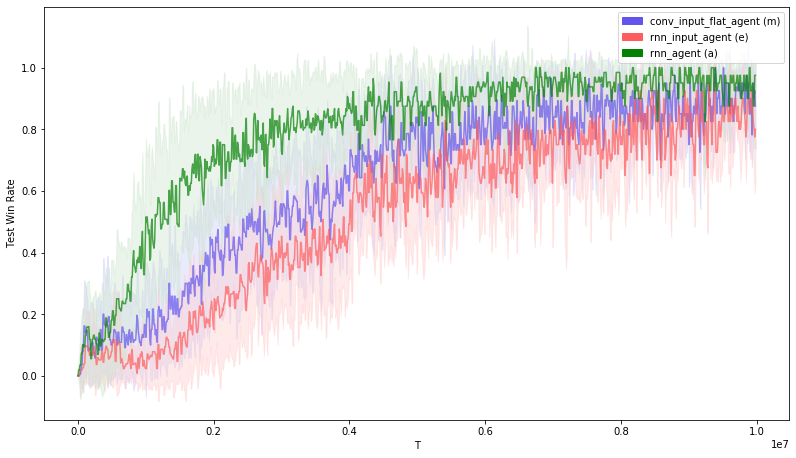
\includegraphics[width=0.45\textwidth]{images/graphs/allagents/2s3z_qmix_1.png}\label{fig:all_agents_2s3z_qmix_a}}
  \hfill
  \subfloat[Test win rate of conv\_input\_grid, conv and rnn architectures.]{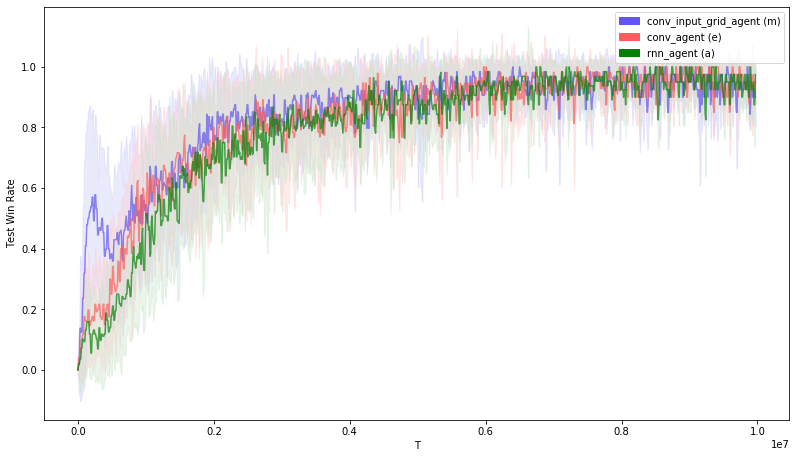
\includegraphics[width=0.45\textwidth]{images/graphs/allagents/2s3z_qmix_2.png}\label{fig:all_agents_2s3z_qmix_b}}
  \caption{Test win rate of each candidate network architecture on the 2s3z map with the QMIX mixing network.}
\end{figure}


\subsubsection{Experiments On Different Grid Sizes}
In this section we experiment with different grid sizes for the inputs of conv\_input\_grid (both the observations and actions as inputs). As described before, this is to determine the best size for training performance: a trade-off is made between the simplicity of a small grid (which has a smaller network that can train more quickly) and the level of detail that can be achieved with a larger grid. 

The map used to experiment upon the grid size is 2s3z (2 Stalkers and 3 Zealots), as this has multiple types of units which must be differentiated upon for the best results.



The grid sizes we will test are 6x6, 12x12, 18x18 and 24x24. As described in section 3.4.2, some simple tests were run to find these batch sizes for the different sizes of grid observations. A memory usage limit of 5Gb (around 40\% of a single GPU's memory) was set to ensure the models can be trained with reasonable resources. The batch sizes were adjusted (for each grid size) to find the maximum batch sizes without exceeding this memory limit. These batch sizes are shown below.



\vspace{3mm}

\begin{tabular}{ |p{3cm}||p{3cm}|p{3cm}|  }
 \hline
 Grid Size& batch\_size&batch\_size\_run\\
 \hline
 6x6   & 32    &8\\
 12x12   & 32    &8\\
 18x18   & 16    &8\\
 24x24   & 12    &8\\
 \hline
\end{tabular}

\vspace{3mm}

The conv\_input\_grid architecture was trained until convergence for each of these grids, and its test win rate was measured at regular intervals (every 20,000 timesteps). For each grid size, the model was trained 5 times to give reproducible results, and allow us to observe the variance in performance. Figure \ref{fig:gridsizes} shows the results of these experiments.


\begin{figure}
    \centering
    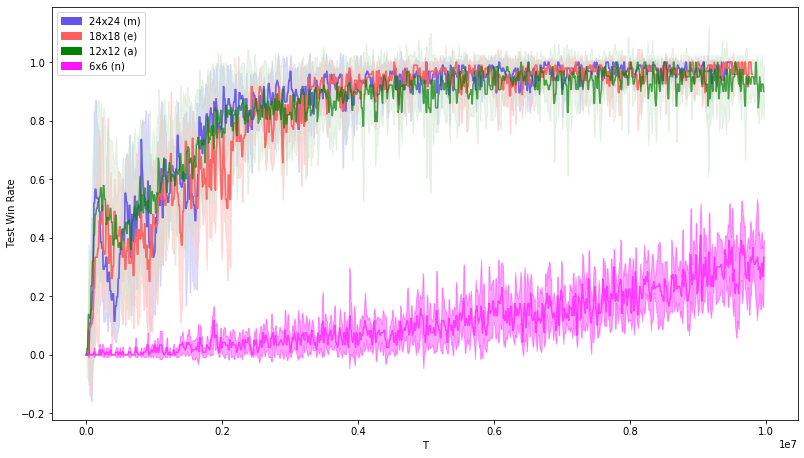
\includegraphics[scale=0.3]{images/graphs/gridsizes/allgrids.png}
    \caption{The test win rate of the conv\_input\_grid architecture with various grid sizes.}
    \label{fig:gridsizes}
\end{figure}

Clearly, the $6 \times 6$ grid performs very poorly: although some learning can be seen to have taken place, little progress and large variance is still apparent after 10,000,000 timesteps. This is likely a result of the grid not being able to represent the complexities of the map well enough: the relations between agents has been abstracted too far away, since 36 cells is not enough to represnt this.

All other sizes performed very similarly. Each size has a very large initial rate of learning (between 0 and 200,000 timesteps), reaching around a $50\%$ test win rate very quickly. From here on, every grid size exhibits a steady increase to its convergence of around $92\%$ test win rate after around 3,000,000 timesteps. The similarity of these results suggest that a grid size of $12 \times 12$ or above is enough to represent the environment effectively.

However, some grid sizes have more variance in there performance at different timesteps. For example, the $24 \times 24$ grid (shown in blue in figure \ref{fig:gridsizes}) has the highest variance before convergence. $12 \times 12$ (shown in green) has particularly low variance at this point. On the other hand, the $24 \times 24$ grid exhibits the lowest variance after convergence, whereas the $12 \times 12$ grid has the largest variance in this timeframe. An explanation for this is that the $24 \times 24$ grid was trained with a smaller batch size. This inherently introduces more noise into the gradient descent steps, increasing variance as it is trained. However, once it converges, the size of the grid allows for a very detailed abstraction of the environment, so gives more stable performance.

\subsection{Architecture Independent of Number of Units}
In this section we run experiments to evaluate the viability of an agent network that is independent of the number of units on the map. As described in the Methodology section, this was achieved by removing the agent id input from the conv\_input\_grid, since this input was the only input or output affected by the number of units on the map. The architecture yielded is referred to ad conv\_input\_grid\_no\_id.


An experiment is conducted for this new architecture in the same way as before: the architecture is trained until convergence, with regular testing to evaluate the performance over time. Again, 5 of these experiments are run to ensure reproducility.

Figure \ref{fig:noid} shows the results of this experiments compared to the previous results for the conv\_input\_grid architecture.

\begin{figure}
    \centering
    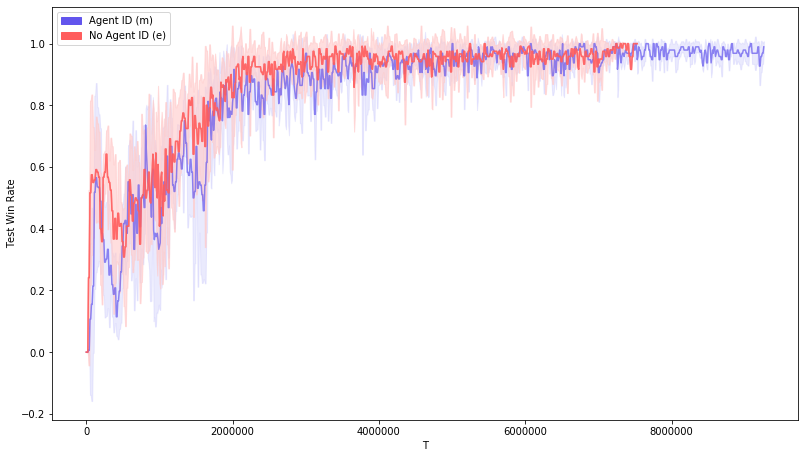
\includegraphics[scale=0.3]{images/graphs/NoId/noid.png}
    \caption{The test win rate of the conv\_input\_grid and conv\_input\_grid\_no\_id architectures.}
    \label{fig:noid}
\end{figure}


Clearly, the performance of both architectures is extremely clear. In fact, surprisingly, the conv\_input\_grid\_no\_id architecture exhibits slightly higher performance at each timestep, and even converges earlier than the original architecture. 


\sbsection{Refining the Architecture}

In order to refine the conv\_input\_grid\_no\_id architecture, we shall evaluate performance by iteratively stripping away features of the architecture until we see a drop in performance, allowing us to conclude the importance of said features. All experiments in this section take place on the 2s3z map with the QMIX mixing network, and with the same environment parameters as before.

\subsubsection{RNN Importance}
We first compare the conv\_input\_grid architecture with and without the GRU-cell, which makes the architecture recurrent. The non-RNN architecture is produced by simply removing the GRU cell, so that there is simply two fully connected linear layers after ther convolutional encoder (with a ReLU between them). The results of this experiment can be seen in figure \ref{fig:rnn_vs_no_rnn}.

\begin{figure}
    \centering
    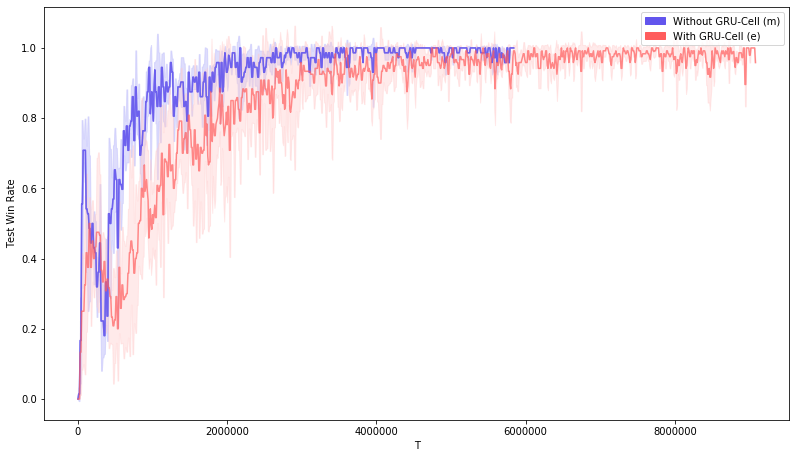
\includegraphics[scale=0.3]{images/graphs/observations/rnn_vs_non_rnn.png}
    \caption{The test win rate of the conv\_input\_grid architecture with and without a GRU-cell.}
    \label{fig:rnn_vs_no_rnn}
\end{figure}

Surprisingly, the architecture without a GRU-cell performed best, converging more quickly (although both architectures exhibited a similar maximum test win rate of 95+\%. This can be explained by the deterministic nature of the 2s3z map. Smaller maps in the environment (such as 2s3z) are very deterministic, and therefore do not require agents with rnn architectures to be successful. In this example, the simplicity of the network was likely able to converge more quickly.


\subsubsection{Experimenting with Observations}

Due to the success of the conv\_input\_grid architecture with no agent id, we hypothesise that each agent can tell units apart (which is of fundamental importance for the success of micromanagement) by the remaining observations (unit type, health, and if they are an ally or enemy). For example, a team of units may learn to all target the enemy with the lowest health, leading to focus fire on a single agent at a time, which is an effective strategy.

To test this hypothesis, we shall test the agent with different levels of observation, and compare their learning rates. In the standard conv\_input\_grid architecture, the observation contains the agent ID, and for each other unit, their health, unit type and ally or enemy status. 

We have already seen success in an agent that does not have agent ID in the observation, so the next step is to remove data from the observation until a noticeable difference in performance is seen. The performance of these architectures can be seen in figure \ref{fig:observations_a}. As a control measure, the architecture was also tested with an empty observation, shown in figure \ref{fig:observations_b}.

\begin{figure}[!tbp]
  \centering
  \subfloat[]{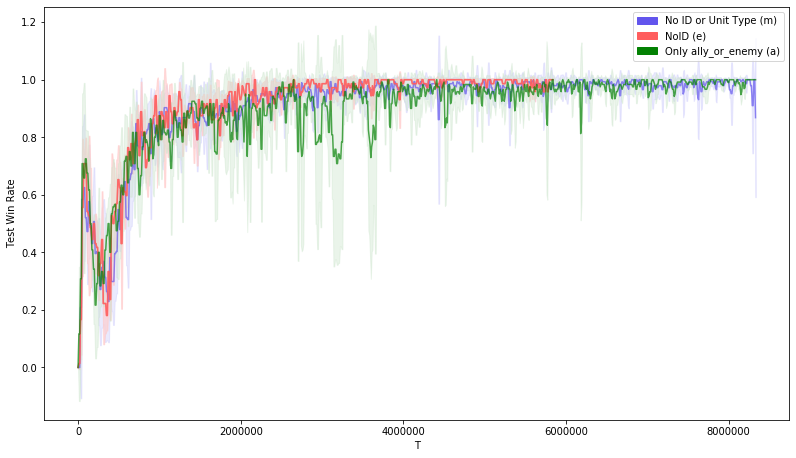
\includegraphics[width=0.45\textwidth]{images/graphs/observations/a.png}\label{fig:observations_a}}
  \hfill
  \subfloat[]{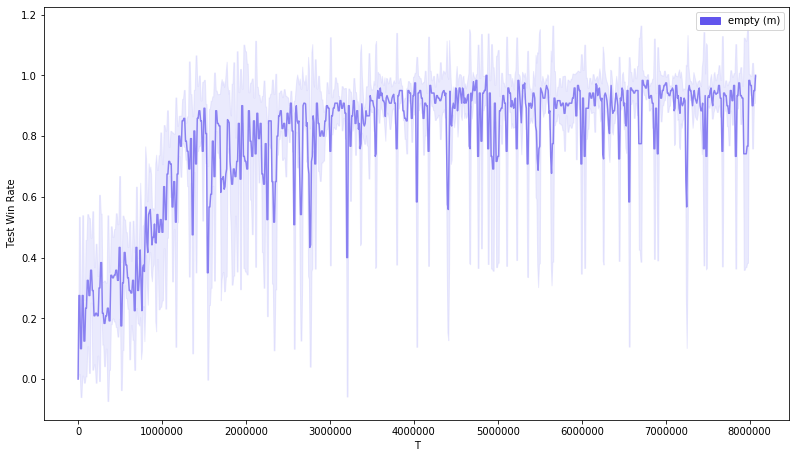
\includegraphics[width=0.45\textwidth]{images/graphs/observations/b.png}\label{fig:observations_b}}
  \caption{Test win rate of the conv\_input\_grid architecture with various levels of observations.}
\end{figure}


Surprisingly, the level of observations used by the network has little effect on performance. The architecture showed similar performance regardless of whether the agent ID or unit type was included, so these observations can be regarded as unnecessary for this architecture in this map. There was increased variance (but similar limit performance) when the health of other units were not included (leaving only the ally\_or\_enemy observation). 

Even more remarkably, the architecture performs fairly well without a single observation, reaching 80+\% limit performance (with large variance). The explanation for this success comes from the representation of available actions, and the fact that they are also passed as an input to the agent. Each available action contains information about the enemy units (since each enemy unit provides an action for attack), as well as the location of the agent with respect to the enemies. The actions are represented by a grid, so this information can easily be encoded into useful obseravtion-like data using the convolutional encoder. The high varianc likely comes from the fact that this is an implicit observation, rather than explicit.

